\documentclass[12pt]{article}
\usepackage[utf8]{inputenc}
\usepackage{geometry}
\geometry{letterpaper, margin=0.25in}
\usepackage{graphicx} 
\usepackage{multicol}
\usepackage{parskip}
\usepackage{booktabs}
\usepackage{array} 
\usepackage{paralist} 
\usepackage{verbatim}
\usepackage{sectsty}
\usepackage[shortlabels]{enumitem}

\usepackage{amsmath}
\usepackage{amssymb}
\usepackage{mathtools}
\usepackage{empheq}
\usepackage{xcolor}
\usepackage{bbm}
\usepackage{tikz}
\usepackage{pgfplots}
\usepackage{tikz-cd}
\usepackage{circuitikz}
\usepackage{multirow}
\pgfplotsset{compat=1.18}
\usetikzlibrary{intersections, decorations.markings}
\tikzset{
    marking along/.style n args={2}{
        decoration={
                markings, 
                mark=at position #1 with {\arrow{#2}}
        },
        postaction={decorate}
        },
    marking along/.default={0.5}{>}
    wavy/.style={
        decorate,decoration={coil,aspect=0}
     },
    two marks/.style n args={1}{
        decoration={
            markings,
            mark=at position 0.25 with {\arrow{#1}},
            mark=at position 0.75 with {\arrow{#1}}
         },
         postaction={decorate}
    }
    two marks/.default={>}
}

\colorlet{mygreen}{green!50!teal}
\colorlet{darkblue}{blue!60!black}

\newcommand{\ans}[1]{\boxed{\text{#1}}}
\newcommand{\vecs}[1]{\langle #1\rangle}
\renewcommand{\hat}[1]{\widehat{#1}}

\renewcommand{\P}{\mathbb{P}}
\newcommand{\R}{\mathbb{R}}
\newcommand{\E}{\mathbb{E}}
\newcommand{\Z}{\mathbb{Z}}
\newcommand{\N}{\mathbb{N}}
\newcommand{\Q}{\mathbb{Q}}
\newcommand{\C}{\mathbb{C}}

\newcommand{\ind}{\mathbbm{1}}
\newcommand{\qed}{\quad \blacksquare}

\newcommand{\brak}[1]{\left\langle #1 \right\rangle}
\newcommand{\bra}[1]{\left\langle #1 \right\vert}
\newcommand{\ket}[1]{\left\vert #1 \right\rangle}

\newcommand{\abs}[1]{\left\vert #1 \right\vert}
\newcommand{\mfX}{\mathfrak{X}}
\newcommand{\ep}{\varepsilon}

\newcommand{\Ec}{\mathcal{E}}
\newcommand{\Nc}{\mathcal{N}}
\newcommand{\A}{\mathcal{A}}
\newcommand{\F}{\mathcal{F}}
\newcommand{\Cc}{\mathcal{C}}
\newcommand{\B}{\mathcal{B}}
\newcommand{\M}{\mathcal{M}}
\newcommand{\X}{\chi}
\renewcommand{\L}{\mathcal{L}}

\newcommand{\sub}{\subseteq}
\newcommand{\st}{\text{ s.t. }}
\newcommand{\card}{\text{card }}
\renewcommand{\div}{\vspace*{10pt}\hrule\vspace*{10pt}}
\newcommand{\surj}{\twoheadrightarrow}
\newcommand{\inj}{\hookrightarrow}
\newcommand{\biject}{\hookrightarrow \hspace{-8pt} \rightarrow}
\renewcommand{\bar}[1]{\overline{#1}}
\newcommand{\overcirc}[1]{\overset{\circ}{#1}}
\newcommand{\diam}{\text{diam }}
\newcommand{\iid}{\overset{	ext{iid}}{\sim}}

\renewcommand{\Re}{\text{Re}\,}
\renewcommand{\Im}{\text{Im}\,}
\newcommand{\Var}{\text{Var}\,}
\newcommand{\Cov}{\text{Cov}\,}

\DeclareMathOperator*{\argmax}{\arg\max}
\DeclareMathOperator*{\argmin}{\arg\min}

\newcommand{\sign}{\text{sign}\,}

\newcommand*{\tbf}[1]{\ifmmode\mathbf{#1}\else\textbf{#1}\fi}

\usepackage{tcolorbox}
\tcbuselibrary{breakable, skins}
\tcbset{enhanced}
\newenvironment*{tbox}[2][gray]{
    \begin{tcolorbox}[
        parbox=false,
        colback=#1!5!white,
        colframe=#1!75!black,
        breakable,
        title={#2}
    ]}
    {\end{tcolorbox}}

\newenvironment*{exercise}[2][red]{
    \begin{tcolorbox}[
        parbox=false,
        colback=#1!5!white,
        colframe=#1!75!black,
        breakable,
        title={#2}
    ]}
    {\end{tcolorbox}}

\newenvironment*{proof}[1][blue]{
\begin{tcolorbox}[
    parbox=false,
    colback=#1!5!white,
    colframe=#1!75!black,
    breakable
]}
{\end{tcolorbox}}
\newenvironment*{proposition}[1][gray]{
    \begin{tcolorbox}[
        parbox=false,
        colback=#1!5!white,
        colframe=#1!75!black,
        breakable
    ]}
    {\end{tcolorbox}}


\begin{document}
\begin{multicols}{2}
    \begin{flushleft}
        \parbox{0.5\textwidth}{\Large ENGN 1931Y: Homework 1}
    \end{flushleft}
    \begin{flushright}
        \tbf{Milan Capoor}\\
        26 September 2026
    \end{flushright}
\end{multicols}
\div

\section*{Problem 1 --- 10 points}
    Draw a component block diagram for each of the following feedback control systems:
    \begin{enumerate}[a.]
        \item The manual steering system of an automobile
        
    \color{darkblue}
        \begin{center}
        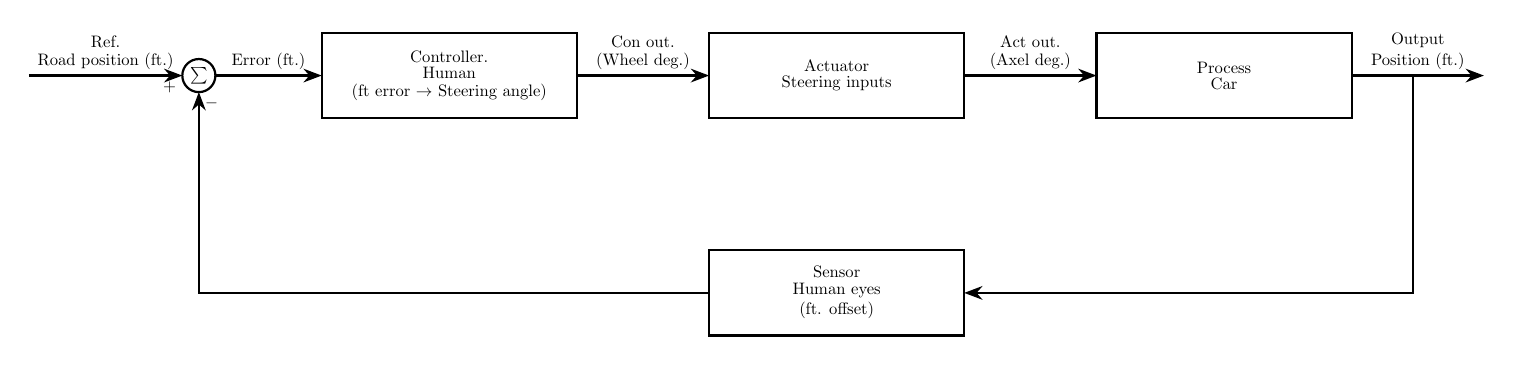
\begin{tikzpicture}[>=Stealth, thick, scale=0.6, every node/.style={transform shape}, font=\normalsize]
            \draw (0,0) circle (0.35) node[midway] {$\sum$};
            \draw[->] (-3.6,0) -- (-0.35,0) node[midway, above] {\shortstack{\textcolor{black}{Ref}. \\ Road position (ft.)}} node[below left] {$+$};

            \draw[->] (0.35,0) -- (2.6,0) node[midway, above] {Error (ft.)};

            \draw (2.6,-0.9) rectangle ++(5.4,1.8) node[midway] {\shortstack{\textcolor{black}{Controller}. \\ Human\\ (ft error $\to$ Steering angle)}};
            \draw[->] (8.0,0) -- (10.8,0) node[midway, above] {\shortstack{\textcolor{black}{Con out.} \\ (Wheel deg.)}};

            \draw (10.8,-0.9) rectangle ++(5.4,1.8) node[midway] {\shortstack{\textcolor{black}{Actuator} \\ Steering inputs}};
            \draw[->] (16.2,0) -- (19.0,0) node[midway, above] {\shortstack{\textcolor{black}{Act out.} \\ (Axel deg.)}};

            \draw (19.0,-0.9) rectangle ++(5.4,1.8) node[midway] {\shortstack{\textcolor{black}{Process} \\ Car}};
            \draw[->] (24.4,0) -- (27.2,0) node[midway, above] {\shortstack{\textcolor{black}{Output} \\ Position (ft.)}};

            \draw[->] (25.7,0) -- (25.7,-4.6) -- (16.2,-4.6);
            \draw (10.8,-5.5) rectangle ++(5.4,1.8) node[midway] {\shortstack{\textcolor{black}{Sensor} \\ Human eyes \\(ft. offset)}};
            \draw[->] (10.8,-4.6) -- (0,-4.6) -- (0,-0.35) node[below right] {$-$};
        \end{tikzpicture}
        \end{center}
    \color{black}


        \item The water level controlled by a float and valve

        \color{blue}
        \begin{center}
        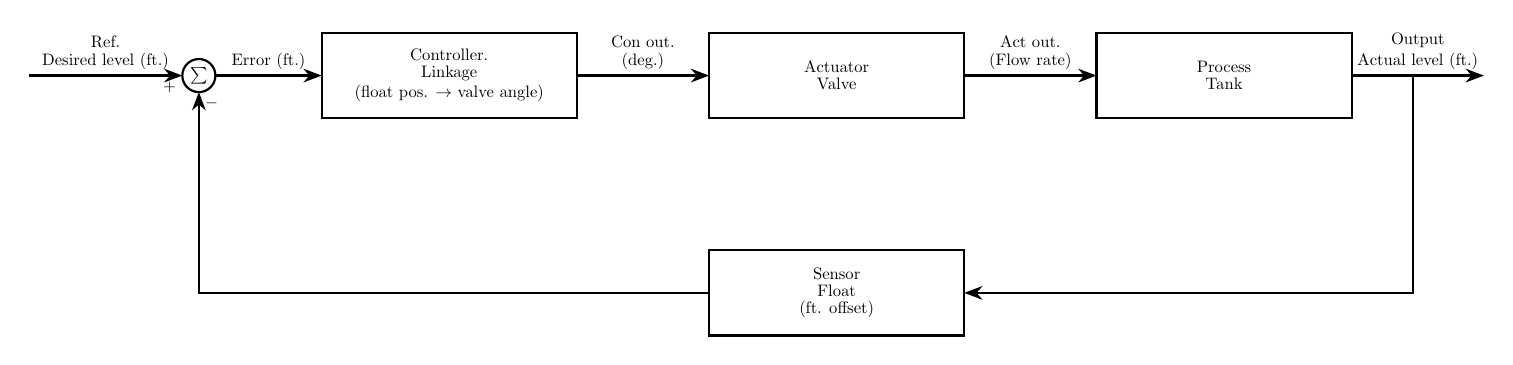
\begin{tikzpicture}[>=Stealth, thick, scale=0.6, every node/.style={transform shape}, font=\normalsize]
            \draw (0,0) circle (0.35) node[midway] {$\sum$};
            \draw[->] (-3.6,0) -- (-0.35,0) node[midway, above] {\shortstack{\textcolor{black}{Ref}. \\ Desired level (ft.)}} node[below left] {$+$};

            \draw[->] (0.35,0) -- (2.6,0) node[midway, above] {Error (ft.)};

            \draw (2.6,-0.9) rectangle ++(5.4,1.8) node[midway] {\shortstack{\textcolor{black}{Controller}. \\ Linkage\\ (float pos. $\to$ valve angle)}};
            \draw[->] (8.0,0) -- (10.8,0) node[midway, above] {\shortstack{\textcolor{black}{Con out.} \\ (deg.)}};

            \draw (10.8,-0.9) rectangle ++(5.4,1.8) node[midway] {\shortstack{\textcolor{black}{Actuator} \\ Valve}};
            \draw[->] (16.2,0) -- (19.0,0) node[midway, above] {\shortstack{\textcolor{black}{Act out.} \\ (Flow rate)}};

            \draw (19.0,-0.9) rectangle ++(5.4,1.8) node[midway] {\shortstack{\textcolor{black}{Process} \\ Tank}};
            \draw[->] (24.4,0) -- (27.2,0) node[midway, above] {\shortstack{\textcolor{black}{Output} \\ Actual level (ft.)}};

            \draw[->] (25.7,0) -- (25.7,-4.6) -- (16.2,-4.6);
            \draw (10.8,-5.5) rectangle ++(5.4,1.8) node[midway] {\shortstack{\textcolor{black}{Sensor} \\ Float \\(ft. offset)}};
            \draw[->] (10.8,-4.6) -- (0,-4.6) -- (0,-0.35) node[below right] {$-$};
        \end{tikzpicture}
        \end{center}
        \color{black}

        \item Temperature control in a refrigerator
        
          \color{darkblue}
        \begin{center}
        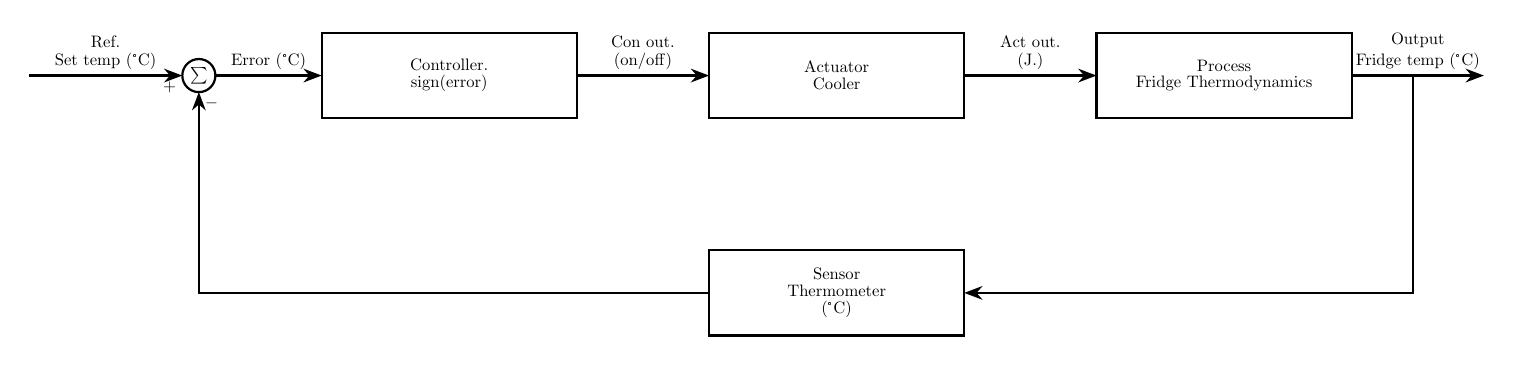
\begin{tikzpicture}[>=Stealth, thick, scale=0.6, every node/.style={transform shape}, font=\normalsize]
            \draw (0,0) circle (0.35) node[midway] {$\sum$};
            \draw[->] (-3.6,0) -- (-0.35,0) node[midway, above] {\shortstack{\textcolor{black}{Ref}. \\ Set temp (°C)}} node[below left] {$+$};

            \draw[->] (0.35,0) -- (2.6,0) node[midway, above] {Error (°C)};

            \draw (2.6,-0.9) rectangle ++(5.4,1.8) node[midway] {\shortstack{\textcolor{black}{Controller}. \\ sign(error)}};
            \draw[->] (8.0,0) -- (10.8,0) node[midway, above] {\shortstack{\textcolor{black}{Con out.} \\ (on/off)}};

            \draw (10.8,-0.9) rectangle ++(5.4,1.8) node[midway] {\shortstack{\textcolor{black}{Actuator} \\ Cooler}};

            \draw[->] (16.2,0) -- (19.0,0) node[midway, above] {\shortstack{\textcolor{black}{Act out.} \\ (J.)}};

            \draw (19.0,-0.9) rectangle ++(5.4,1.8) node[midway] {\shortstack{\textcolor{black}{Process} \\ Fridge Thermodynamics}};

            \draw[->] (24.4,0) -- (27.2,0) node[midway, above] {\shortstack{\textcolor{black}{Output} \\ Fridge temp (°C)}};

            \draw[->] (25.7,0) -- (25.7,-4.6) -- (16.2,-4.6);
            \draw (10.8,-5.5) rectangle ++(5.4,1.8) node[midway] {\shortstack{\textcolor{black}{Sensor} \\ Thermometer \\(°C)}};

            \draw[->] (10.8,-4.6) -- (0,-4.6) -- (0,-0.35) node[below right] {$-$};
        \end{tikzpicture}
        \end{center}
    \color{black}

        \item Watt's steam engine with fly-ball governor

           \color{darkblue}
        \begin{center}
        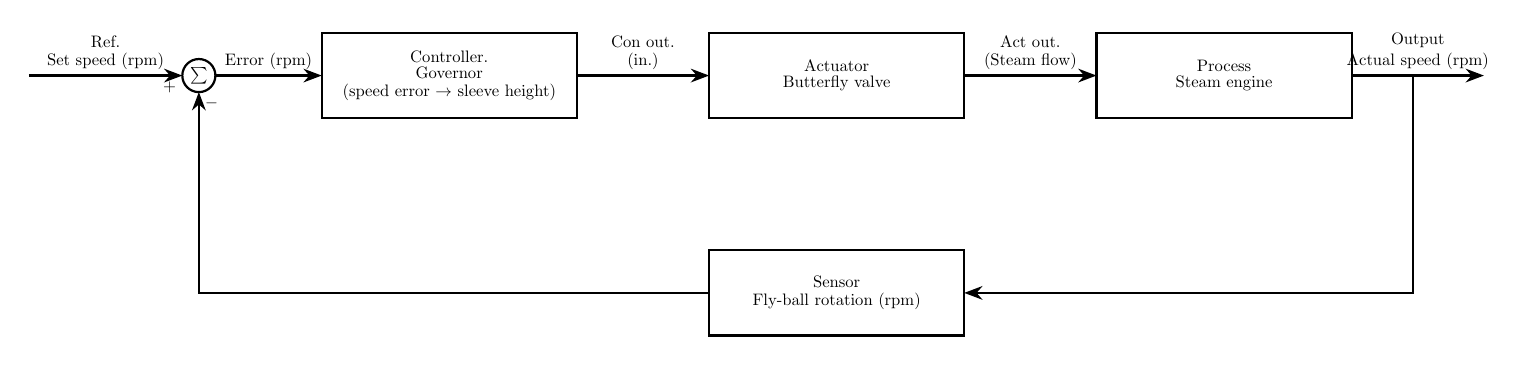
\begin{tikzpicture}[>=Stealth, thick, scale=0.6, every node/.style={transform shape}, font=\normalsize]
            \draw (0,0) circle (0.35) node[midway] {$\sum$};
            \draw[->] (-3.6,0) -- (-0.35,0) node[midway, above] {\shortstack{\textcolor{black}{Ref}. \\ Set speed (rpm)}} node[below left] {$+$};

            \draw[->] (0.35,0) -- (2.6,0) node[midway, above] {Error (rpm)};

            \draw (2.6,-0.9) rectangle ++(5.4,1.8) node[midway] {\shortstack{\textcolor{black}{Controller}. \\ Governor\\ (speed error $\to$ sleeve height)}};
            \draw[->] (8.0,0) -- (10.8,0) node[midway, above] {\shortstack{\textcolor{black}{Con out.} \\ (in.)}};

            \draw (10.8,-0.9) rectangle ++(5.4,1.8) node[midway] {\shortstack{\textcolor{black}{Actuator} \\ Butterfly valve}};

            \draw[->] (16.2,0) -- (19.0,0) node[midway, above] {\shortstack{\textcolor{black}{Act out.} \\ (Steam flow)}};

            \draw (19.0,-0.9) rectangle ++(5.4,1.8) node[midway] {\shortstack{\textcolor{black}{Process} \\ Steam engine}};

            \draw[->] (24.4,0) -- (27.2,0) node[midway, above] {\shortstack{\textcolor{black}{Output} \\ Actual speed (rpm)}};

            \draw[->] (25.7,0) -- (25.7,-4.6) -- (16.2,-4.6);
            \draw (10.8,-5.5) rectangle ++(5.4,1.8) node[midway] {\shortstack{\textcolor{black}{Sensor} \\ Fly-ball rotation (rpm)}};

            \draw[->] (10.8,-4.6) -- (0,-4.6) -- (0,-0.35) node[below right] {$-$};
        \end{tikzpicture}
        \end{center}
    \color{black}
    \end{enumerate}


    \begin{center}
        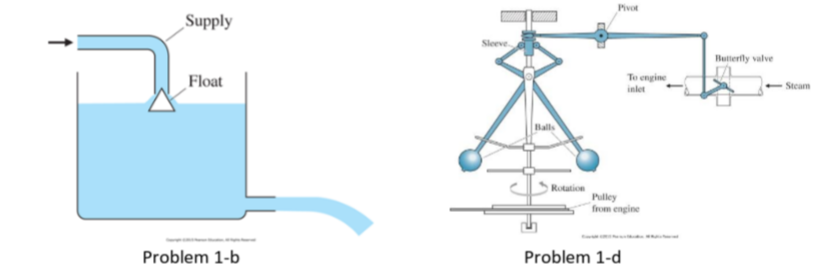
\includegraphics[width=0.8\textwidth]{p1.png}
    \end{center}

    In each case indicate the location of the elements listed below and give the units associated with each signal:
    \begin{itemize}
        \item The process
        \item The process desired output signal
        \item The sensor
        \item The actuator \& actuator output signal
        \item The controller \& controller output signal
        \item The reference signal
        \item The error signal
    \end{itemize}




\section*{Problem 2 --- 10 points}
    A machine for making paper is diagrammed below. There are two main parameters under feedback control: the density of fibers, as controlled by the consistency of the thick stock that flows from the headbox onto the wire, and the moisture content of the final product that comes out of the dryers. Stock from the machine chest is diluted by the white water returning from under the wire, as controlled by a control valve (CV).

    \begin{center}
        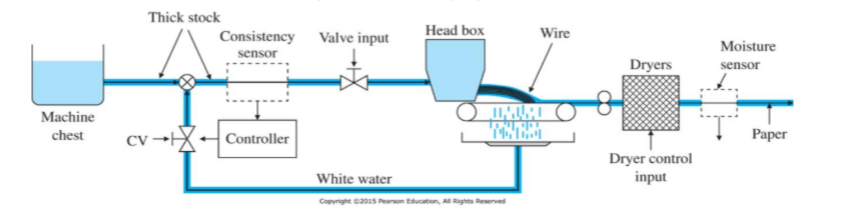
\includegraphics[width=0.8\textwidth]{p2.png}
    \end{center}

    A meter supplies a reading of the consistency. At the ``dry end'' of the machine, there is a moisture sensor. Draw a block diagram and identify the components listed in Problem 1 (the process, etc.) for the following:
    \begin{enumerate}[a.]
        \item Control of consistency
        
        \color{darkblue}
            \begin{center}
            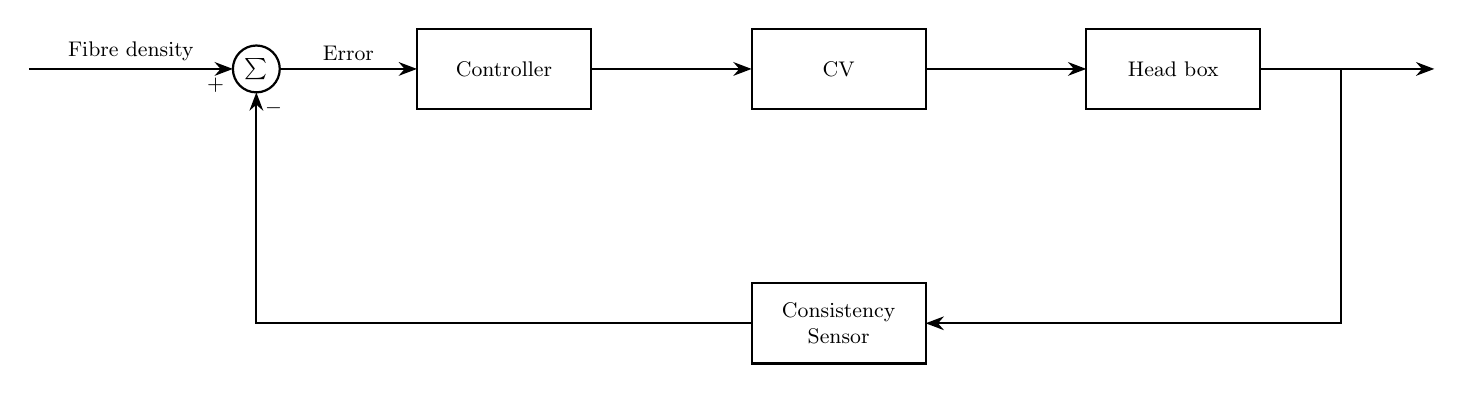
\begin{tikzpicture}[>=Stealth, thick, scale=0.85, every node/.style={transform shape}, font=\small]
                \draw (0,0) circle (0.35) node[midway] {$\sum$};
                \draw[->] (-3.4,0) -- (-0.35,0) node[midway, above] {Fibre density} node[below left] {$+$};
                
                \draw[->] (0.35,0) -- (2.4,0) node[midway, above] {Error};
                
                \draw (2.4,-0.6) rectangle ++(2.6,1.2) node[midway] {Controller};
                \draw[->] (5,0) -- (7.4,0);
                
                \draw (7.4,-0.6) rectangle ++(2.6,1.2) node[midway] {CV};
                \draw[->] (10,0) -- (12.4,0);
                
                \draw (12.4,-0.6) rectangle ++(2.6,1.2) node[midway] {Head box};
                \draw[->] (15,0) -- (17.6,0);
                
                \draw[->] (16.2,0) -- (16.2,-3.8) -- (10,-3.8);
                \draw (7.4,-4.4) rectangle ++(2.6,1.2) node[midway] {\shortstack{Consistency\\ Sensor}};
                \draw[->] (7.4,-3.8) -- (0,-3.8) -- (0,-0.35) node[below right] {$-$};
            \end{tikzpicture}
            \end{center}
        \color{black}

        \item Control of moisture
        \color{darkblue}
        
           \begin{center}
            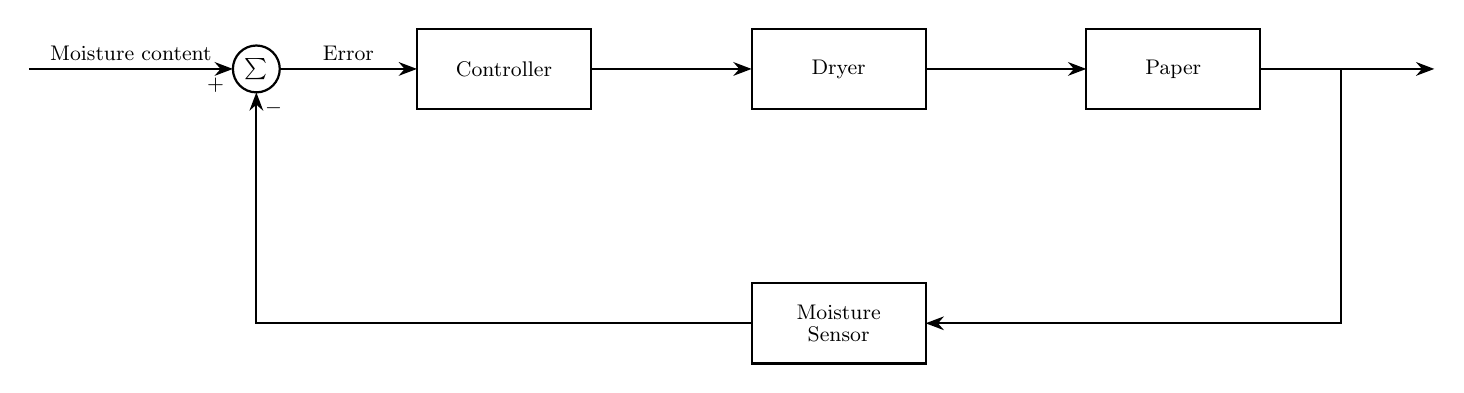
\begin{tikzpicture}[>=Stealth, thick, scale=0.85, every node/.style={transform shape}, font=\small]
                \draw (0,0) circle (0.35) node[midway] {$\sum$};
                \draw[->] (-3.4,0) -- (-0.35,0) node[midway, above] {Moisture content} node[below left] {$+$};
                
                \draw[->] (0.35,0) -- (2.4,0) node[midway, above] {Error};
                
                \draw (2.4,-0.6) rectangle ++(2.6,1.2) node[midway] {Controller};
                \draw[->] (5,0) -- (7.4,0);
                
                \draw (7.4,-0.6) rectangle ++(2.6,1.2) node[midway] {Dryer};
                \draw[->] (10,0) -- (12.4,0);
                
                \draw (12.4,-0.6) rectangle ++(2.6,1.2) node[midway] {Paper};
                \draw[->] (15,0) -- (17.6,0);
                
                \draw[->] (16.2,0) -- (16.2,-3.8) -- (10,-3.8);
                \draw (7.4,-4.4) rectangle ++(2.6,1.2) node[midway] {\shortstack{Moisture\\ Sensor}};
                \draw[->] (7.4,-3.8) -- (0,-3.8) -- (0,-0.35) node[below right] {$-$};
            \end{tikzpicture}
            \end{center}
        \color{black}

    \end{enumerate}

\section*{Problem 3 --- 10 points}
    Find the Laplace transform for the following time functions:
    \begin{enumerate}[a.]
        \item $f(t) = \sin(3t) + 2\cos(3t) + e^{-t}\sin(3t)$
        
        \color{darkblue}
            \[\L[f] = \frac{3}{s^2 + 9} + \frac{6s}{s^2 + 9} + \frac{1}{(s+1)^2 + 9}\]
        \color{black}

        \item $f(t) = t \sin t$
        
        \color{darkblue}
            \[\L[f] = \frac{2s}{(s^2 + 1)^2}\]
        \color{black}

        \item $f(t) = 4 + 7t + t^2 + \delta(t)$
        
        \color{darkblue}
        \[\L[f] = \frac{4}{s} + \frac{7}{s^2} + \frac{2}{s^3} + 1\]
        \color{black}
    \end{enumerate}

\section*{Problem 4 --- 10 points}
    Using the convolution integral, find the step response of the system whose impulse response is given below:
    \[
        h(t) = \begin{cases} 
            t e^{-t} & t \geq 0 \\ 
            0 & t < 0 
        \end{cases}
    \]
    Verify the results using the Laplace transform.

    \color{darkblue}
        \begin{align*}
            y(t) &= \int_{-\infty}^{\infty} u(\tau) h(t - \tau) d\tau \\
            &= \int_{0}^{t} (t - \tau) e^{-(t - \tau)} d\tau \\
            &= e^{-t} \int_{0}^{t} (t - \tau) e^{\tau} d\tau \\
            &= e^{-t} \left[ (t - \tau) e^{\tau} \Big|_{0}^{t} + \int_{0}^{t} e^{\tau} d\tau \right] \\
            &= e^{-t} \left[ 0 - t + (e^{t} - 1) \right] \\
            &= e^{-t} (e^{t} - 1 - t) \\
            &= \boxed{1 - e^{-t} - t e^{-t}}
        \end{align*}

        Or, via Laplace:
        \[\L[h(t)] = H(s) = \frac{1}{(s+1)^2}\]
        so 
        \[Y(s) = H(s) \cdot U(s) = \frac{1}{(s+1)^2} \cdot \frac{1}{s} = \frac{1}{s(s+1)^2}\]
        which is exactly 
        \[\L[ 1 - e^{-t} - t e^{-t}] = \frac{1}{s} -\frac{1}{s + 1} - \frac{1}{(s+1)^2} = \frac{1}{s(s+1)^2}\]
    \color{black}



\section*{Problem 5 --- 10 points}
    Solve the following ODEs using the Laplace transform:
    \begin{enumerate}[a.]
        \item $\ddot{y}(t) + y(t) = t$; \quad $y(0) = 1$; \quad $\dot{y}(0) = -1$
        
        \color{darkblue}
            \begin{gather*}
            \L[\ddot y + y] = \L[t] \\
            s^2 Y(s) - s y(0) - \dot y(0) + Y(s) = \frac{1}{s^2} \\
            (s^2 + 1) Y(s) - s + 1 = \frac{1}{s^2}
        \end{gather*}
        \begin{align*}
            Y(s) &= \frac{1}{s^2(s^2 + 1)} + \frac{s - 1}{s^2 + 1} \\
            &= \frac{1}{s^2} - \frac{1}{s^2 + 1} + \frac{s}{s^2 + 1} - \frac{1}{s^2 + 1}\\ 
            y(t) &= t - \sin t + \cos t - \sin t \\
            &= \boxed{t + \cos t - 2\sin t}
        \end{align*}
        \color{black}

        \item $\ddot{y}(t) + 2\dot{y}(t) = e^t$; \quad $y(0) = 1$; \quad $\dot{y}(0) = 2$
        
        \color{darkblue}
        
        \begin{gather*}
           ( s^2 Y(s) - sy(0) - \dot y(0)) + 2(sY(s) - y(0)) = \frac{1}{s-1} \\
            (s^2 + 2s) Y(s) - (s + 2)y(0) - \dot y(0) = \frac{1}{s-1} \\
            s(s + 2) Y(s) - (s + 2) - 2 = \frac{1}{s-1} \\
            \begin{aligned}
                Y(s) &= \frac{1}{(s-1)s(s+2)} + \frac{s + 4}{s(s+2)}\\ 
                &= -\frac{1}{2s} + \frac{1}{6(s + 2)} + \frac{1}{3(s - 1)} + \frac{2}{s} - \frac{1}{s + 2}\\ 
                y(t) &= -\frac{1}{2} + \frac{1}{6} e^{-2t} + \frac{1}{3} e^{t} + 2 - e^{-2t}\\
                &= \boxed{-\frac{5}{6}e^{-2t} + \frac{1}{3} e^{t} + \frac{3}{2}}
            \end{aligned}
        \end{gather*}
        \color{black}

    \end{enumerate}

\section*{Problem 6 --- 10 points}
    Find the time function corresponding to each of the following Laplace transforms:
    \begin{enumerate}[a.]
        \item $F(s) = \dfrac{3s^2 + 6s + 6}{(s+1)(s^2+6s+10)}$
        
        \color{darkblue}
            \begin{align*}
                F(s) &= \frac{3s^2 + 6s + 6}{(s+1)(s^2+6s+10)}\\ 
                &= \frac{12s}{5(s^2 + 6s + 10)} + \frac{3}{5(s + 1)}\\
                &= \frac{12}{5} \frac{s}{(s+3)^2 + 1} + \frac{3}{5} \frac{1}{s + 1}\\
                &= \frac{12}{5} \left[\frac{s + 3}{(s+3)^2 + 1} - \frac{3}{(s+3)^2 + 1}\right] + \frac{3}{5} \frac{1}{s + 1}\\
                f(t) &= \frac{12}{5} \left[e^{-3t} \cos t - 3e^{-3t} \sin t\right] + \frac{3}{5} e^{-t}\\ 
                &= \boxed{\frac{12}{5}e^{-3t} \left(\cos t - 3\sin t\right) + \frac{3}{5} e^{-t}}
            \end{align*}
        \color{black}

        \item $F(s) = \dfrac{e^{-s}}{s^2}$
        
        \color{darkblue}
            \begin{align*}
                F(s) &= \frac{1}{s^2} e^{-s}\\ 
                f(t) &= \boxed{(t - 1)u(t-1)}
            \end{align*}
        \color{black}

    \end{enumerate}
    \textit{Note: You can use integration tables. Use the MATLAB Symbolic Algebra toolbox for verification.}

\end{document}